%%*************************************************************************
%%
%% Anomaly Detection by Means of Statistical Analysis of the Frequency Spectrum
%% V1.1
%% 2011/12/22
%% by Peter Boraros
%% See http://www.pborky.sk/contact for current contact information.
%%
%%*************************************************************************
%%
%% Legal Notice:
%%
%% This code is offered as-is without any warranty either expressed or
%% implied; without even the implied warranty of MERCHANTABILITY or
%% FITNESS FOR A PARTICULAR PURPOSE! 
%% User assumes all risk.
%%
%% This work by Peter Boraros is licensed under a 
%% Creative Commons Attribution-NonCommercial-ShareAlike 3.0 Unported License.
%% http://creativecommons.org/licenses/by-nc-sa/3.0/
%%
%%*************************************************************************

\documentclass[a4paper,journal]{IEEEtran}

\usepackage{cite}
% \usepackage[nocompress]{cite}
\usepackage{ifpdf}

\ifpdf
\usepackage[pdftex]{graphicx}
\graphicspath{{./img/}}
\DeclareGraphicsExtensions{.pdf}
\else
\usepackage[dvips]{graphicx}
\graphicspath{{./img/}}
\DeclareGraphicsExtensions{.eps}
\fi

\usepackage[cmex10]{amsmath}
\usepackage{amsfonts}
\usepackage{amssymb}
\interdisplaylinepenalty=2500

\usepackage{algorithmic}

\usepackage{array}

\usepackage{mdwmath}
\usepackage{mdwtab}

\usepackage{eqparbox}

\usepackage[hang,small,center,bf]{caption}
% \usepackage[tight,normalsize,sf,SF]{subfigure}
%\usepackage[tight,footnotesize]{subfigure}
\usepackage{subfig}
% \usepackage[caption=false,font=normalsize,labelfont=sf,textfont=sf]{subfig}
% \usepackage[caption=false,font=footnotesize]{subfig}

\usepackage[utf8x]{inputenc}

\usepackage[colorlinks=true,urlcolor=blue]{hyperref}
\usepackage{url}
\usepackage{fixltx2e}
\usepackage{stfloats}
\usepackage{ucs}
\usepackage{multirow}

% correct bad hyphenation here
\hyphenation{op-tical net-works semi-conduc-tor}

\renewcommand{\labelitemi}{$\bullet$}
\renewcommand{\labelitemii}{$\circ$}
\renewcommand{\labelitemiii}{$\ast$}

\setlength{\textheight}{260mm}

\begin{document}

\title{Anomaly Detection by Means of Analysis of the Frequency Spectrum}
\date{March 11, 2012}
\author{Peter~Boráros %
\thanks{{Peter Boráros}, see~{\scriptsize\url{http://www.pborky.sk/contact}} for a contact infomation}}%%

% The paper headers
%\markboth{Peter Boráros, Czech technical university, Faculty of Electrical Engineering, Prague, Czech Republic}{}

\IEEEcompsoctitleabstractindextext{%
\begin{abstract}
This article provides information about analysis of the frequency spectrum of a computer network traffic.
The computer network traffic can be seen as an sequence of events occuring in time domain. This ought to be 
transformed to the frequency domain and then a statistical model of particular behaviors ought to be found. 
The model is then usable to statistical inference and recognition of some security problems in computer network.
\end{abstract}}

\maketitle
\IEEEdisplaynotcompsoctitleabstractindextext
\IEEEpeerreviewmaketitle

\section{Introduction}\label{intro}
Motivation for this work is to enable ability to distinguish a periodic behavior of potential threats from ordinary
network communication. Dataset that has been provided for purposes of this work contains an agregate information of 
about one day of the network communication as well as the information of malignancy of particular communication 
participants. The crucial moment of this research is to differentiate an malicious peer-to-peer communication from
other not-malicous classes (especially www proxy servers or DNS servers).

Section \ref{sec:prep} provides formal information about data capturing, and process of extracting features involving 
fourier transformation. Section \ref{sec:experiments} provides owerview of the experiments with testing dataset performed.

\section{Data preparation}\label{sec:prep}
\subsection{Network traffic, gathering the data}
It is possible to represent a network traffic by set of flows distributed in time. The flow is a sequence of packets having  similar attributes. Packets are exchanged usually among network endpoints. Attributes taken under consideration are at least: source and destination endpoint address, port and protocol. Mentioned attributes usualy delimitate flows.

In order to evaluate anomaly rate of paticular flow other properties ought to be taken in account. Especially number of packets and bytes, starting and ending time (time-stamp of the first or the last packet in the flow).

%TODO mention the features 
The time distribution of flows can be determined by considering the starting timestamp of each flow. This approach provides generalized view on the flow, as it has been occured in network channel with unlimited throughput.

Experimental dataset provided for purposes of this work has been extended with classification information, a knowledge if particular endpoint is harmfull or not or even if it is suspicious.

\subsection{Data binning}
In order to reduce minor observation errors binning technique ought to be used. The time axis is divided into disjoint intervals - bins. Let $h$ be number of bins and $\mathbb{F}$ be the set of all flows captured in time interval $\mathbb{T} = (0, T_{max}\rangle $. The $t$-th bin is known as  set of flows $\mathbb{F}_t$ that occurs in time interval $\mathbb{T}_t = ((t-1)\cdot \delta, t\cdot \delta\rangle $ where $t \in \{1, .. h\}$ and $\delta$ is the width of time intervals denoted $\delta = \frac{T_{max}}{h}$. Denote
\begin{equation}
\mathbb{F}_t = \{f : f \in \mathbb{F} \wedge s(f) \in \mathbb{T}_t \}
\end{equation}
where function $s:\mathbb{F} \rightarrow \mathbb{N} $ 
returns starting timestamp of the flow $f\in \mathbb{F}$.

For each interval,
representative value is calculated. Following formula have been considered:
\begin{equation}\label{eq:represent}
r_t = \frac{\sum\limits_{f\in \mathbb{F}_t}b(f)}{\sum\limits_{f\in \mathbb{F}_t}p(f)}
\end{equation}
where $r_t$ is representative of time interval $t$, $\mathbb{F}_t$ is set of flows captured in time 
interval $t$, function $b:\mathbb{F} \rightarrow \mathbb{N}$ outputs size of the flow $f$ in bytes and function 
$p:\mathbb{F} \rightarrow \mathbb{N}$ outputs the packet count of the flow $f$. 
In the other words, value $r_t$ is an average packet size. 

Tuples $s_i = (r_a, \ldots, r_b)$ are ordered lists of representatives for
$a = (i-1)\cdot w +1 $, $b = i\cdot w $ and $ i = 1, \ldots, \lfloor \frac{h-w}{w} \rfloor$,
where $w$ is size of each tuple and $h$ is number of bins. In other words, sequence $r_1,\ldots,r_h$
is chopped into non-overlapping subsequences $s_i$.


%TODO further description of representatives and features

\subsection{Fourier transformation}
Tuples $s_i$ are to be transformed from the time domain to the frequency domain.
This can be achieved by fourier-related tranforms, e.g. by a fourier or a wavelet transform.
The wavelet transform, unlike the fourier transform, captures
not only a notion of the frequency content of the input, by
examining it at different scales, but also temporal content.

To achieve fast computation, a fast fourier transform (FFT) algorithm has been involved.
It is an efficient algorithm to compute the discrete fourier tranform (DFT) and its inverse.
A DFT decomposes a sequence of values into components of different frequencies. 
This operation is useful in many fields but computing it directly from the definition is often 
too slow to be practical.
An FFT is a way to compute the same result more quickly: 
computing a DFT of N points in the naive way, using the definition, takes $O(N^2$) arithmetical 
operations, while an FFT can compute the same result in only $ O(N \log N)$ operations.

The sequence of $N$ complex numbers $x_0, ..., x_{N−1}$ is transformed into the
sequence of $N$ complex numbers $X_0, ..., X_{N−1}$ by the DFT according to the
formula:
\begin{equation}
X_k = \sum_{n=0}^{N-1} x_n e^{-\frac{2 \pi i}{N} k n} \quad \quad k = 0, \dots, N-1
\end{equation}
where $i$ is imaginary unit and $e^{-\frac{2 \pi i}{N} k n}$ is $N$-th root of unity.

The transform is sometimes denoted as 
$\mathcal{F}\colon\mathbb{C}^N \to \mathbb{C}^N$, e.g.
$\mathbf{X} = \mathcal{F} \left ( \mathbf{x} \right )$.

Fourier transform is appliend on sequences $s_i$ resulting in sequences of complex coeficients.
By discarding phase information real coeficients are obtained.
Coeficients are organised in matrix $\mathcal{S}$. Columns of matrix $\mathcal{S}$ are denoted:

\begin{equation}
\mathcal{S}_{*,j} = \mid\mathcal{F}(s_{j})\mid
\end{equation}

An experimental dataset contains also classification information. For particular classes,
different matrices ought to be constructed, specifying the class information in upper index, 
e.g.: $\mathcal{S}^{(c)}$.


\begin{table}[b!]
\begin{center}
\caption{True positive rate of given methods for particular annotations}
\begin{tabular}{r|rr}
Traffic/Feature & feature \ref{eq:first} &  feature \ref{eq:sec} \\ \hline
CMP gateway & 0.3394 & 0.2301\\
dns & 0.4483 & 0.3669\\
FILTER\_MALICIOUS & 0.6774 & 0.7532\\
horizontal scan & 0.5614 & 0.7308 \\
horizontal scan response & 0.2784 & 0.4471\\
Malicious & 0.1931 & 0.1621\\
malware SpyEye request & 0.8429 & 0.8731\\
malware SpyEye response & 0.0000 & 0.0008 \\
p2p & 0.1315 & 0.0335 \\
p2p like & 0.2764 & 0.3211\\
p2p like dest & 0.0623 & 0.0750\\
p2p response & 0.0522 & 0.0619\\
Peashooter & 0.2815 & 0.3319\\
scan sql & 0.7044 & 0.9177\\
skype supernode & 0.2505 & 0.4851\\
skype supernode dest. & 0.1363 & 0.1522 \\
ssh cracking & 0.2391 & 0.4481 \\
ssh cracking response & 0.5974 & 0.5352\\
unknown & 0.1451 & 0.0452\\
vertical scan & 0.0000 & 0.5472\\
\end{tabular}
\end{center}
\label{tbl:tp}
\end{table}

\section{Experiments}\label{sec:experiments}
\subsection{Methods}
Anomaly level, denote $\alpha$, is number from interval $\alpha \in \langle0, 1\rangle$.
For experimental purposes following methods have been tested.
At first for all endpoint $e$ matrix of fourier coeficients $\mathcal{S}^{(e)}$ has been calculated, 
where $e$ denotes endpoint. 
The aggregation over source endpoints has been choosen. That
applies to the formula \ref{eq:represent}.
Only modification to formulas from previos section is that \textit{hanning} windowing function
has been  applied before the fourier transform and as the fourier coeficients are symmetric 
half has been discarded.

Standard deviation  has been calculated columnwise on $\mathcal{S}^{(e)}$ resulting in time-sequence of values.
Then the overall deviation, denote $l^{(e)} $, has been calculated over a time span approx. 25 minutes
as well as over a tail subsequence representing last 5 minutes, denote this as $s^{(e)} $.

One choice used the value $l^{(e)} $ as quantification of particular endpoint.
After obtaining value for all endpoints normalization over is performed, and the anomaly level of each endpoint is
\begin{equation}\label{eq:first}
\alpha^{(e)} = \frac{\max_x l^{(x)} - l^{(e)}}{\max_x l^{(x)} - \min_x l^{(x)}} 
\end{equation}

The other choice took absolute value   of the difference of both values
as quantification of particular endpoint - 
\[a^{(e)} = \mid s^{(e)} - l^{(e)} \mid \].
Related anomaly level of each endpoint is
\begin{equation}\label{eq:sec}
\alpha^{(e)} = \frac{\max_x a^{(x)} - a^{(e)}}{\max_x a^{(x)} - \min_x a^{(x)}}
\end{equation}

Here the $x$ goes over all endpoints.

\subsection{Evaluation}
The {fig. \ref{fig:norm}} shows ROC curves for feature \ref{eq:first} explained above and the {fig. \ref{fig:magic}} 
does the same for feature \ref{eq:sec} . Table \ref{tbl:tp} enlists true positive values of two mentioned methods.

\section{Conclusion}
None given yet. Sorry.
%Simple experiments described above are not the goal of the research.
%Further research of model finding and checking is intended to be done. 
%Next experiments will employ gaussian mixture models along with the EM algorithm. 
%The goal is, to work out  an easy-to-use and fast method for searching and especially for testing 
% multivariate mixture models.



%\begin{thebibliography}{1}
%
%\bibitem{Bor04}
%  \textsc{S. Borman}. (2004). \emph{The Expectation Maximization Algorithm - A short tutorial}.
%  
%\bibitem{Nar03}
%  \textsc{I. Narsky}. (2003). \emph{Goodness of Fit: What Do We Really Want to Know?}. 
%  paper at PHYSTAT2003. SLAC National Accelerator Laboratory. 
%
%\bibitem{Ros62}
%  \textsc{J. Rosenblatt}. (1962). \emph{Note on Multivariate Goodness-of-fit Tests}. 
%  The Annals of Mathematical Statistics 33. 807-810.
%
%\bibitem{KanHar95}
%  \textsc{T. Kanungo, R. N. Haralick}. (1995). 
%  \emph{Multivariate hypotesis testing for Gaussian Data: Theory and Software}.
%
%\bibitem{Ste74}
%  \textsc{M. A. Stephens}. (1974). 
%  \emph{EDF Statistics for Goodness of Fit and Some Comparisons}.
%  Journal of the American Statistical Association 69. 730–737.
%
%\bibitem{Bro08}
%  \textsc{A.E. Brockwell}. (2008). 
%  \emph{Universal Residuals: A Multivariate Transformation}.
%  Statistics \& Probability Letters. 77. 1473-1478.
%
%\bibitem{BicBre83}
%   \textsc{J. Bickel, L. Breiman}. (1983). 
%   \emph{Sums of Functions of Nearest Neighbor Distances, Moment Bounds, Limit Theorems and a Goodness of Fit Test}.
%   The Annals of Probability 11. 185-214. 
%
%
%\end{thebibliography}

\onecolumn

\begin{figure}[t!]%
  \centering
  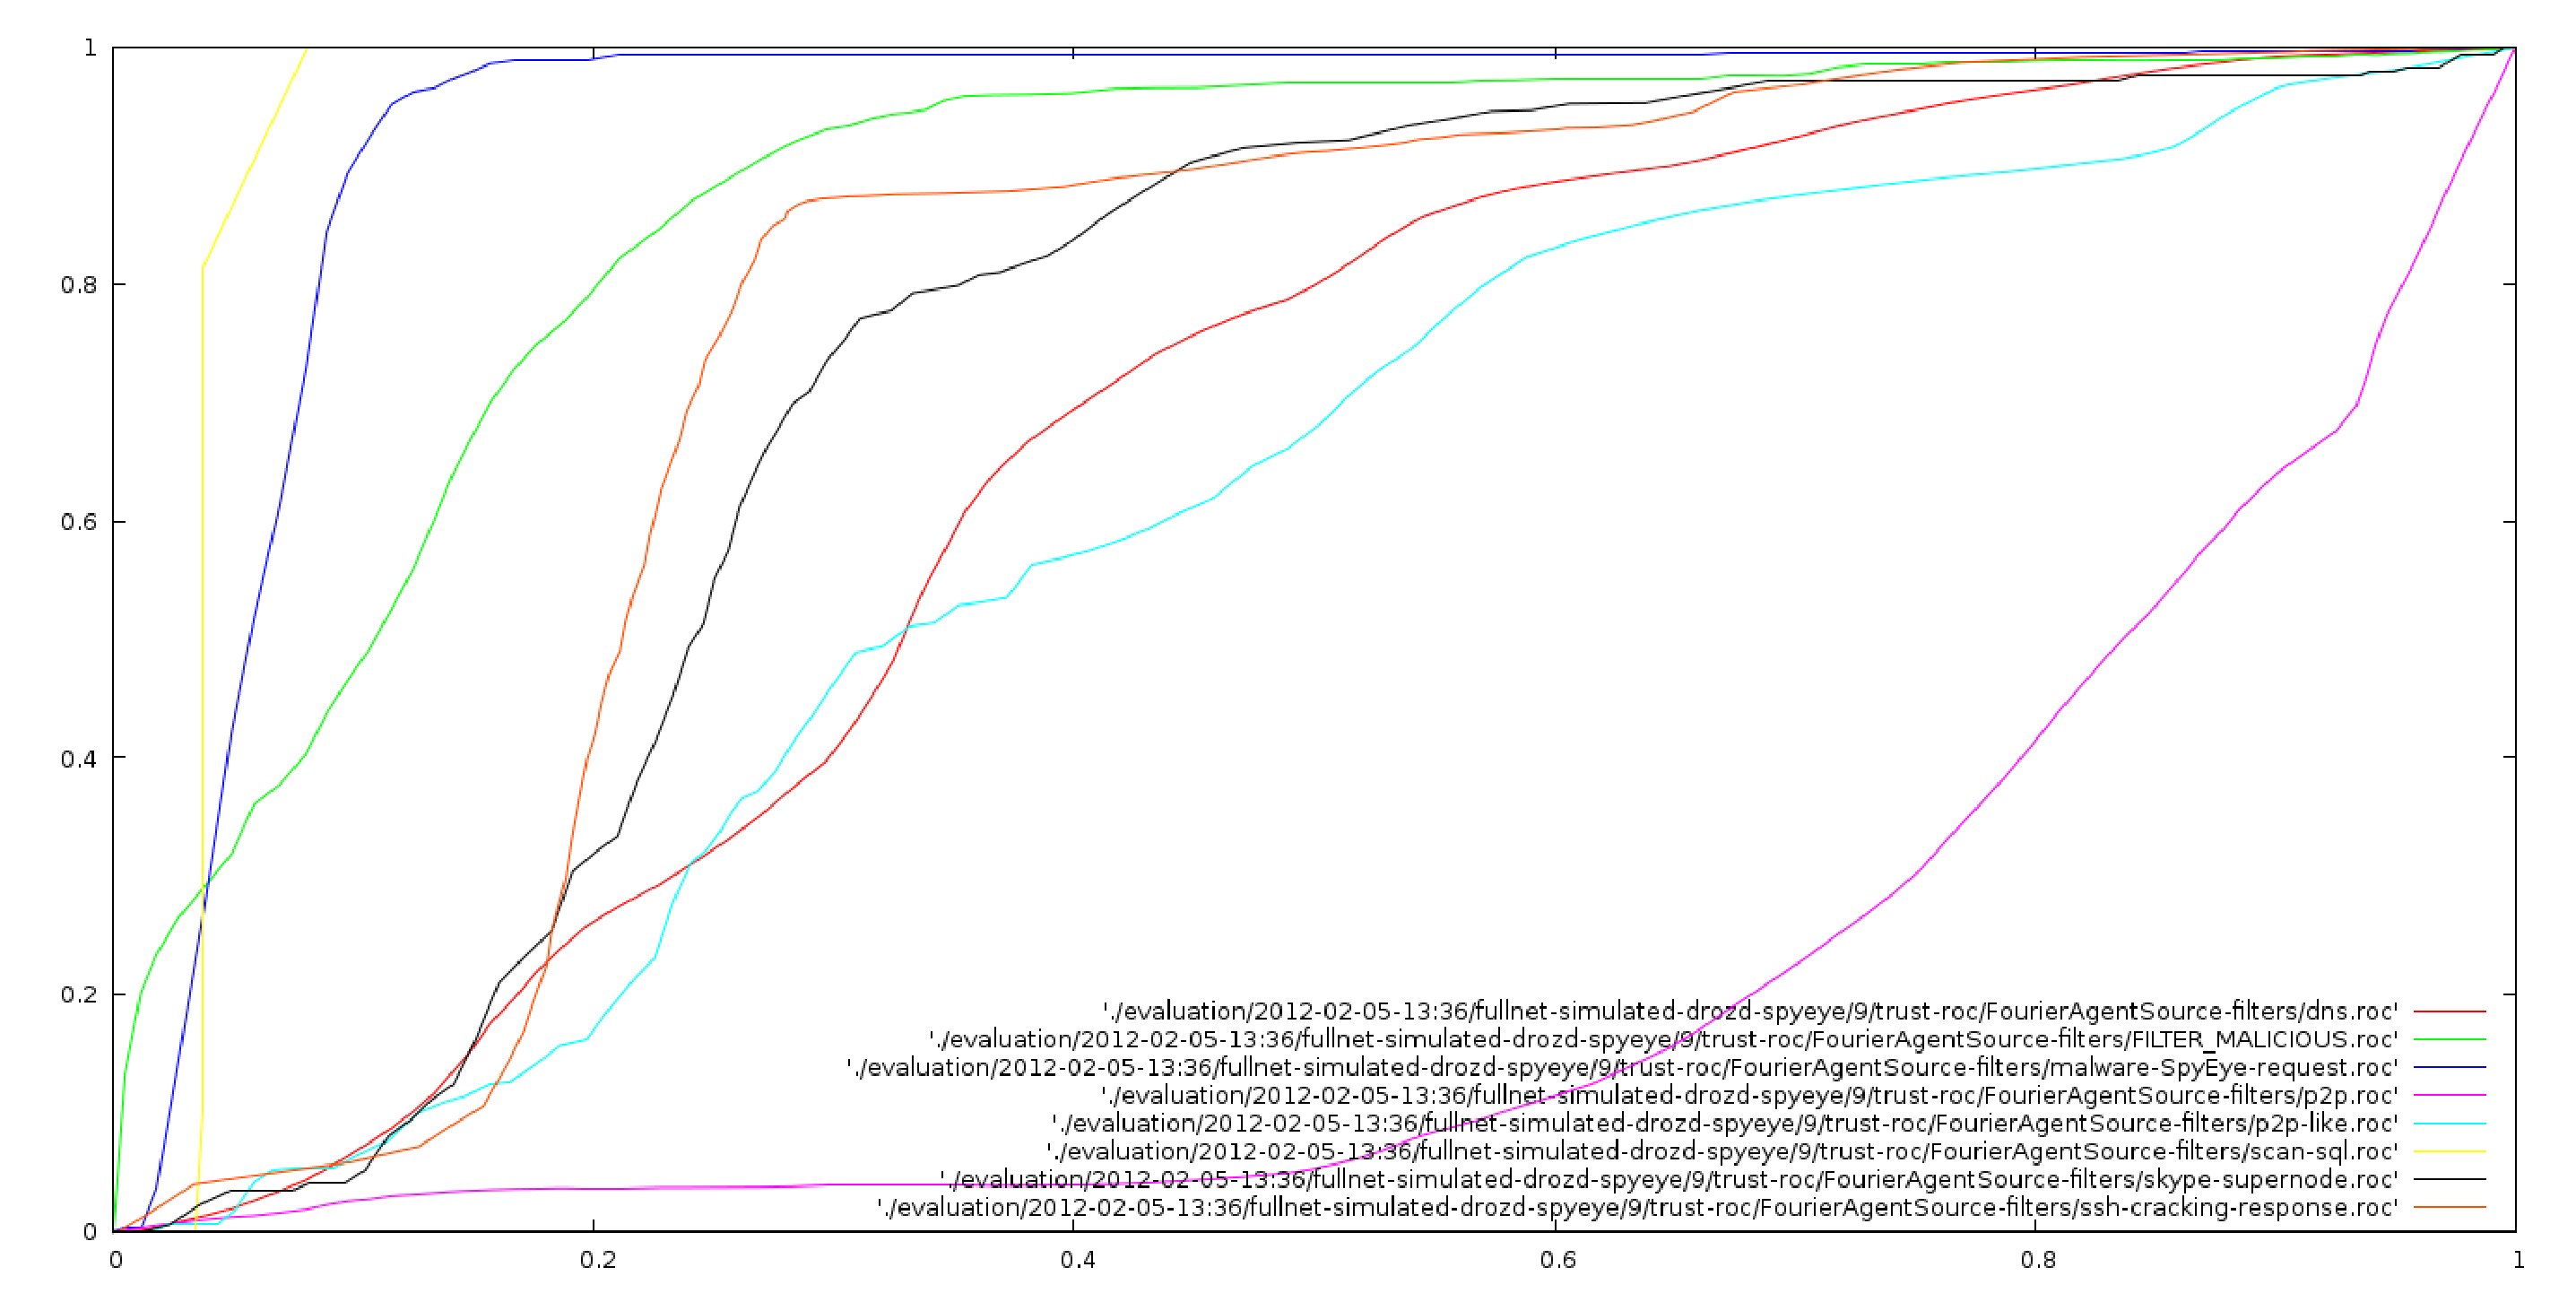
\includegraphics[width=160mm]{norm}
  \caption{ROC curves of the feature \ref{eq:first} matched against known annontanions}
  \label{fig:norm}
\end{figure}


\begin{figure}[t!]%
  \centering
  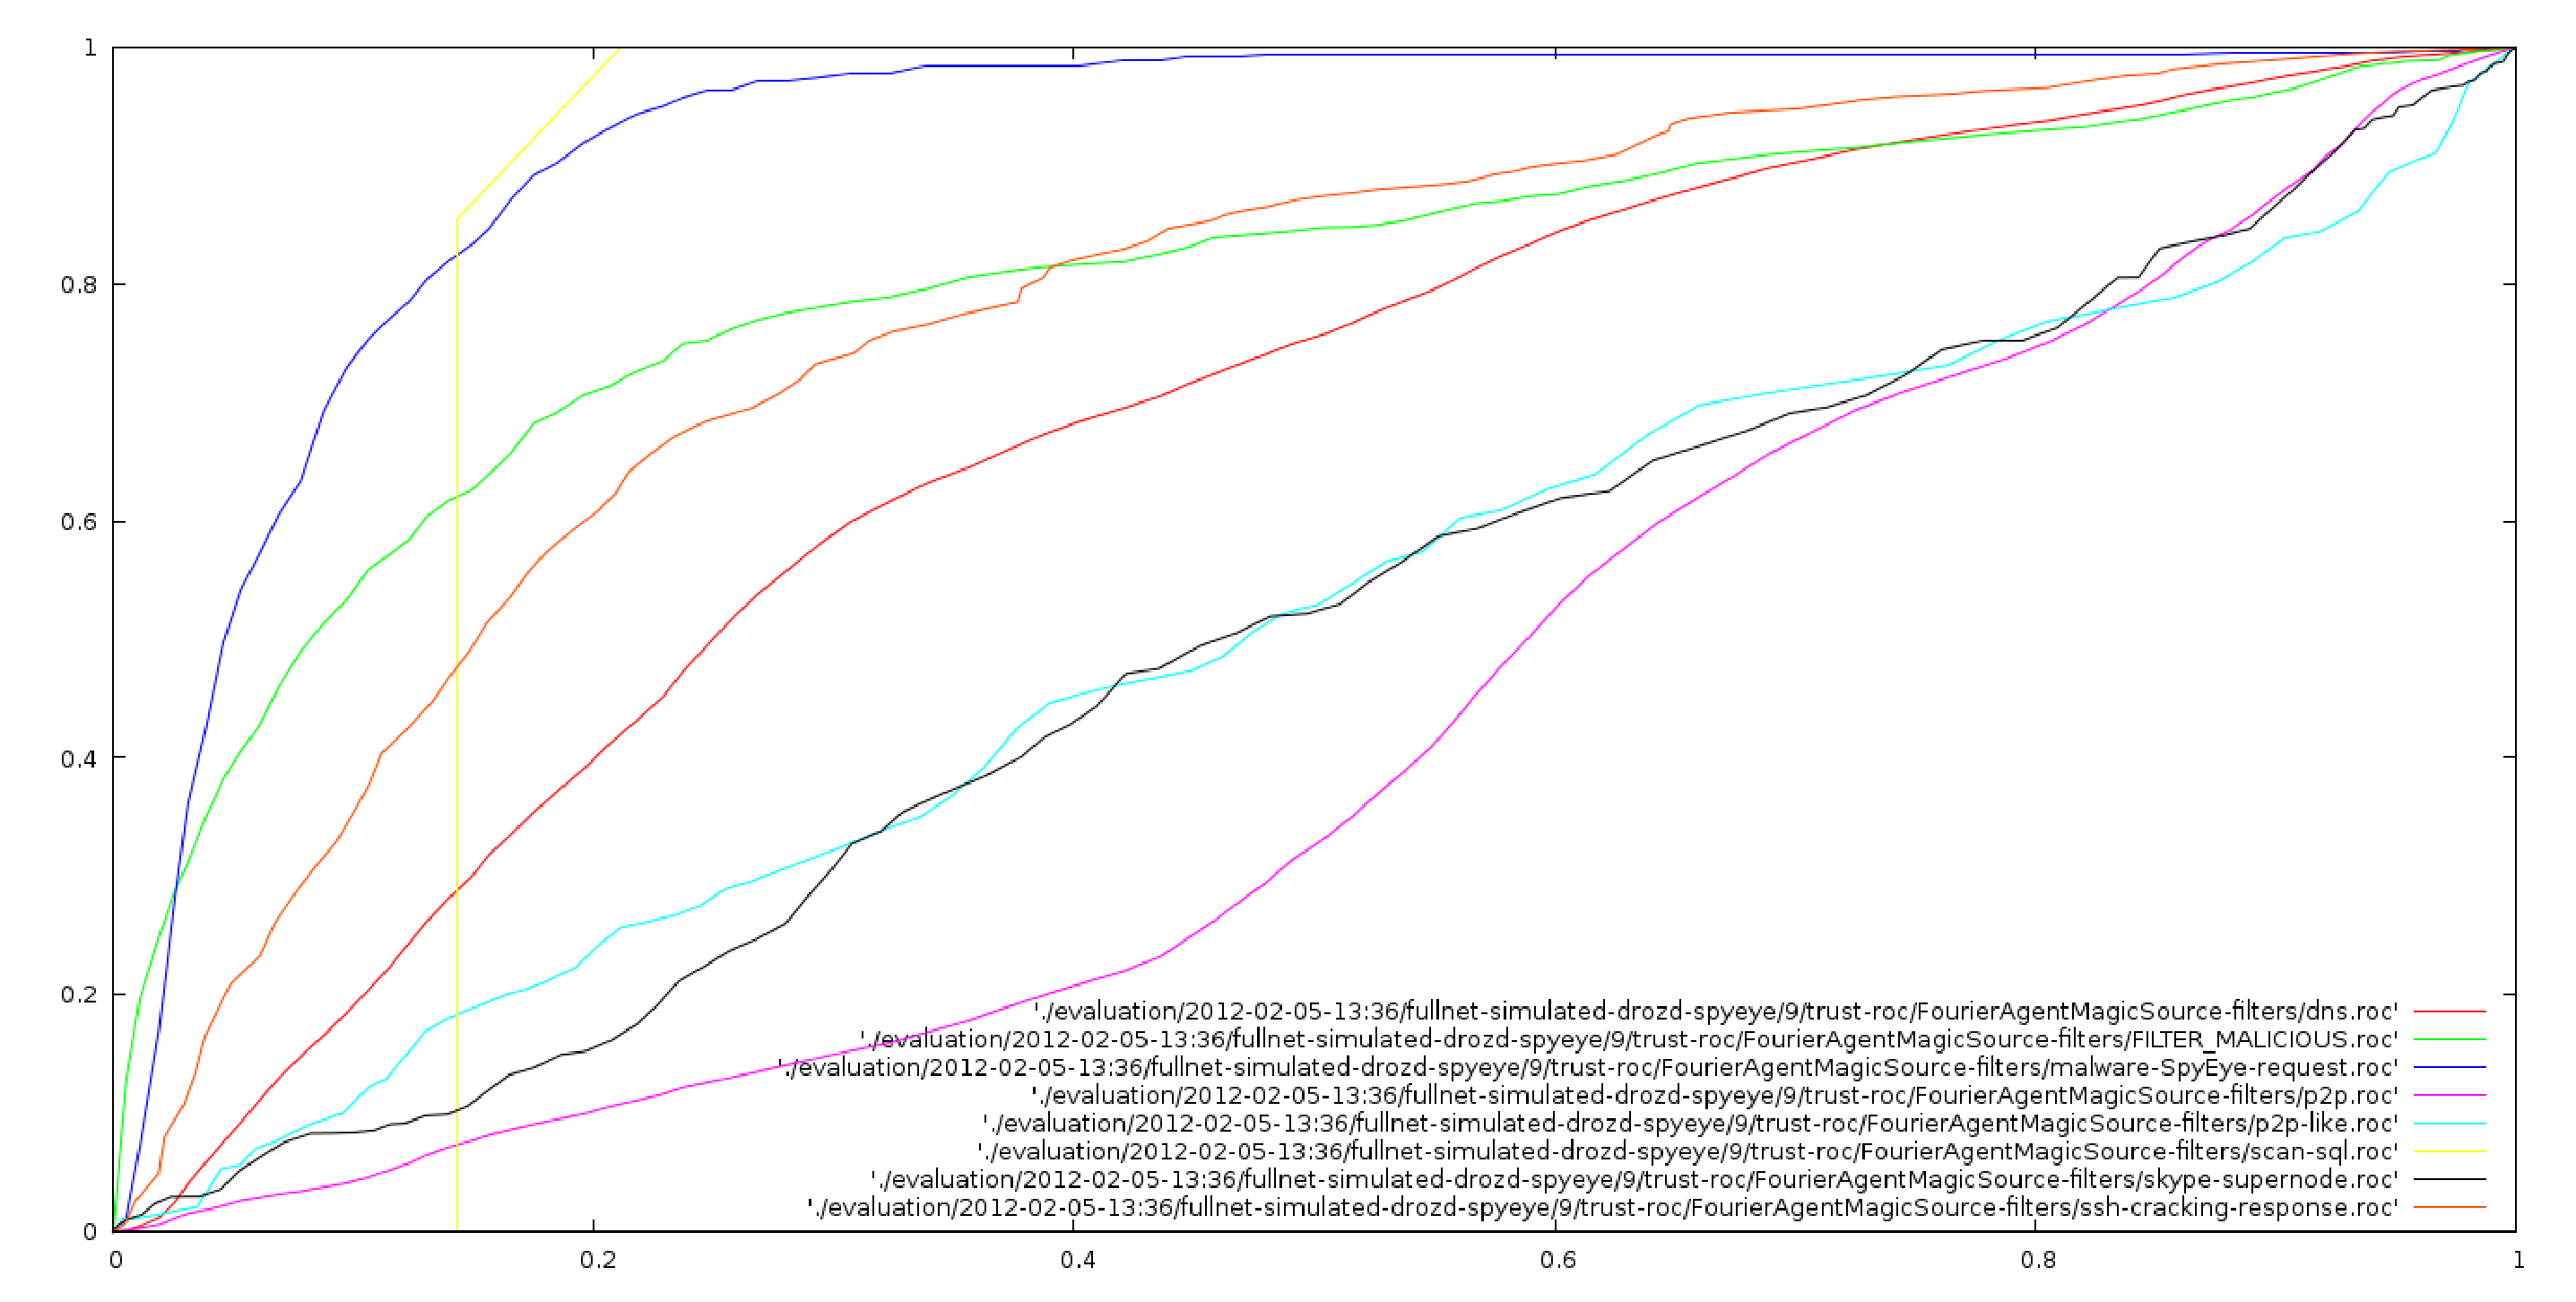
\includegraphics[width=160mm]{magic}
  \caption{ROC curves of the feature \ref{eq:sec} matched against known annontanions}
  \label{fig:magic}
\end{figure}

%\begin{figure}[t!]%
%  \centering
%  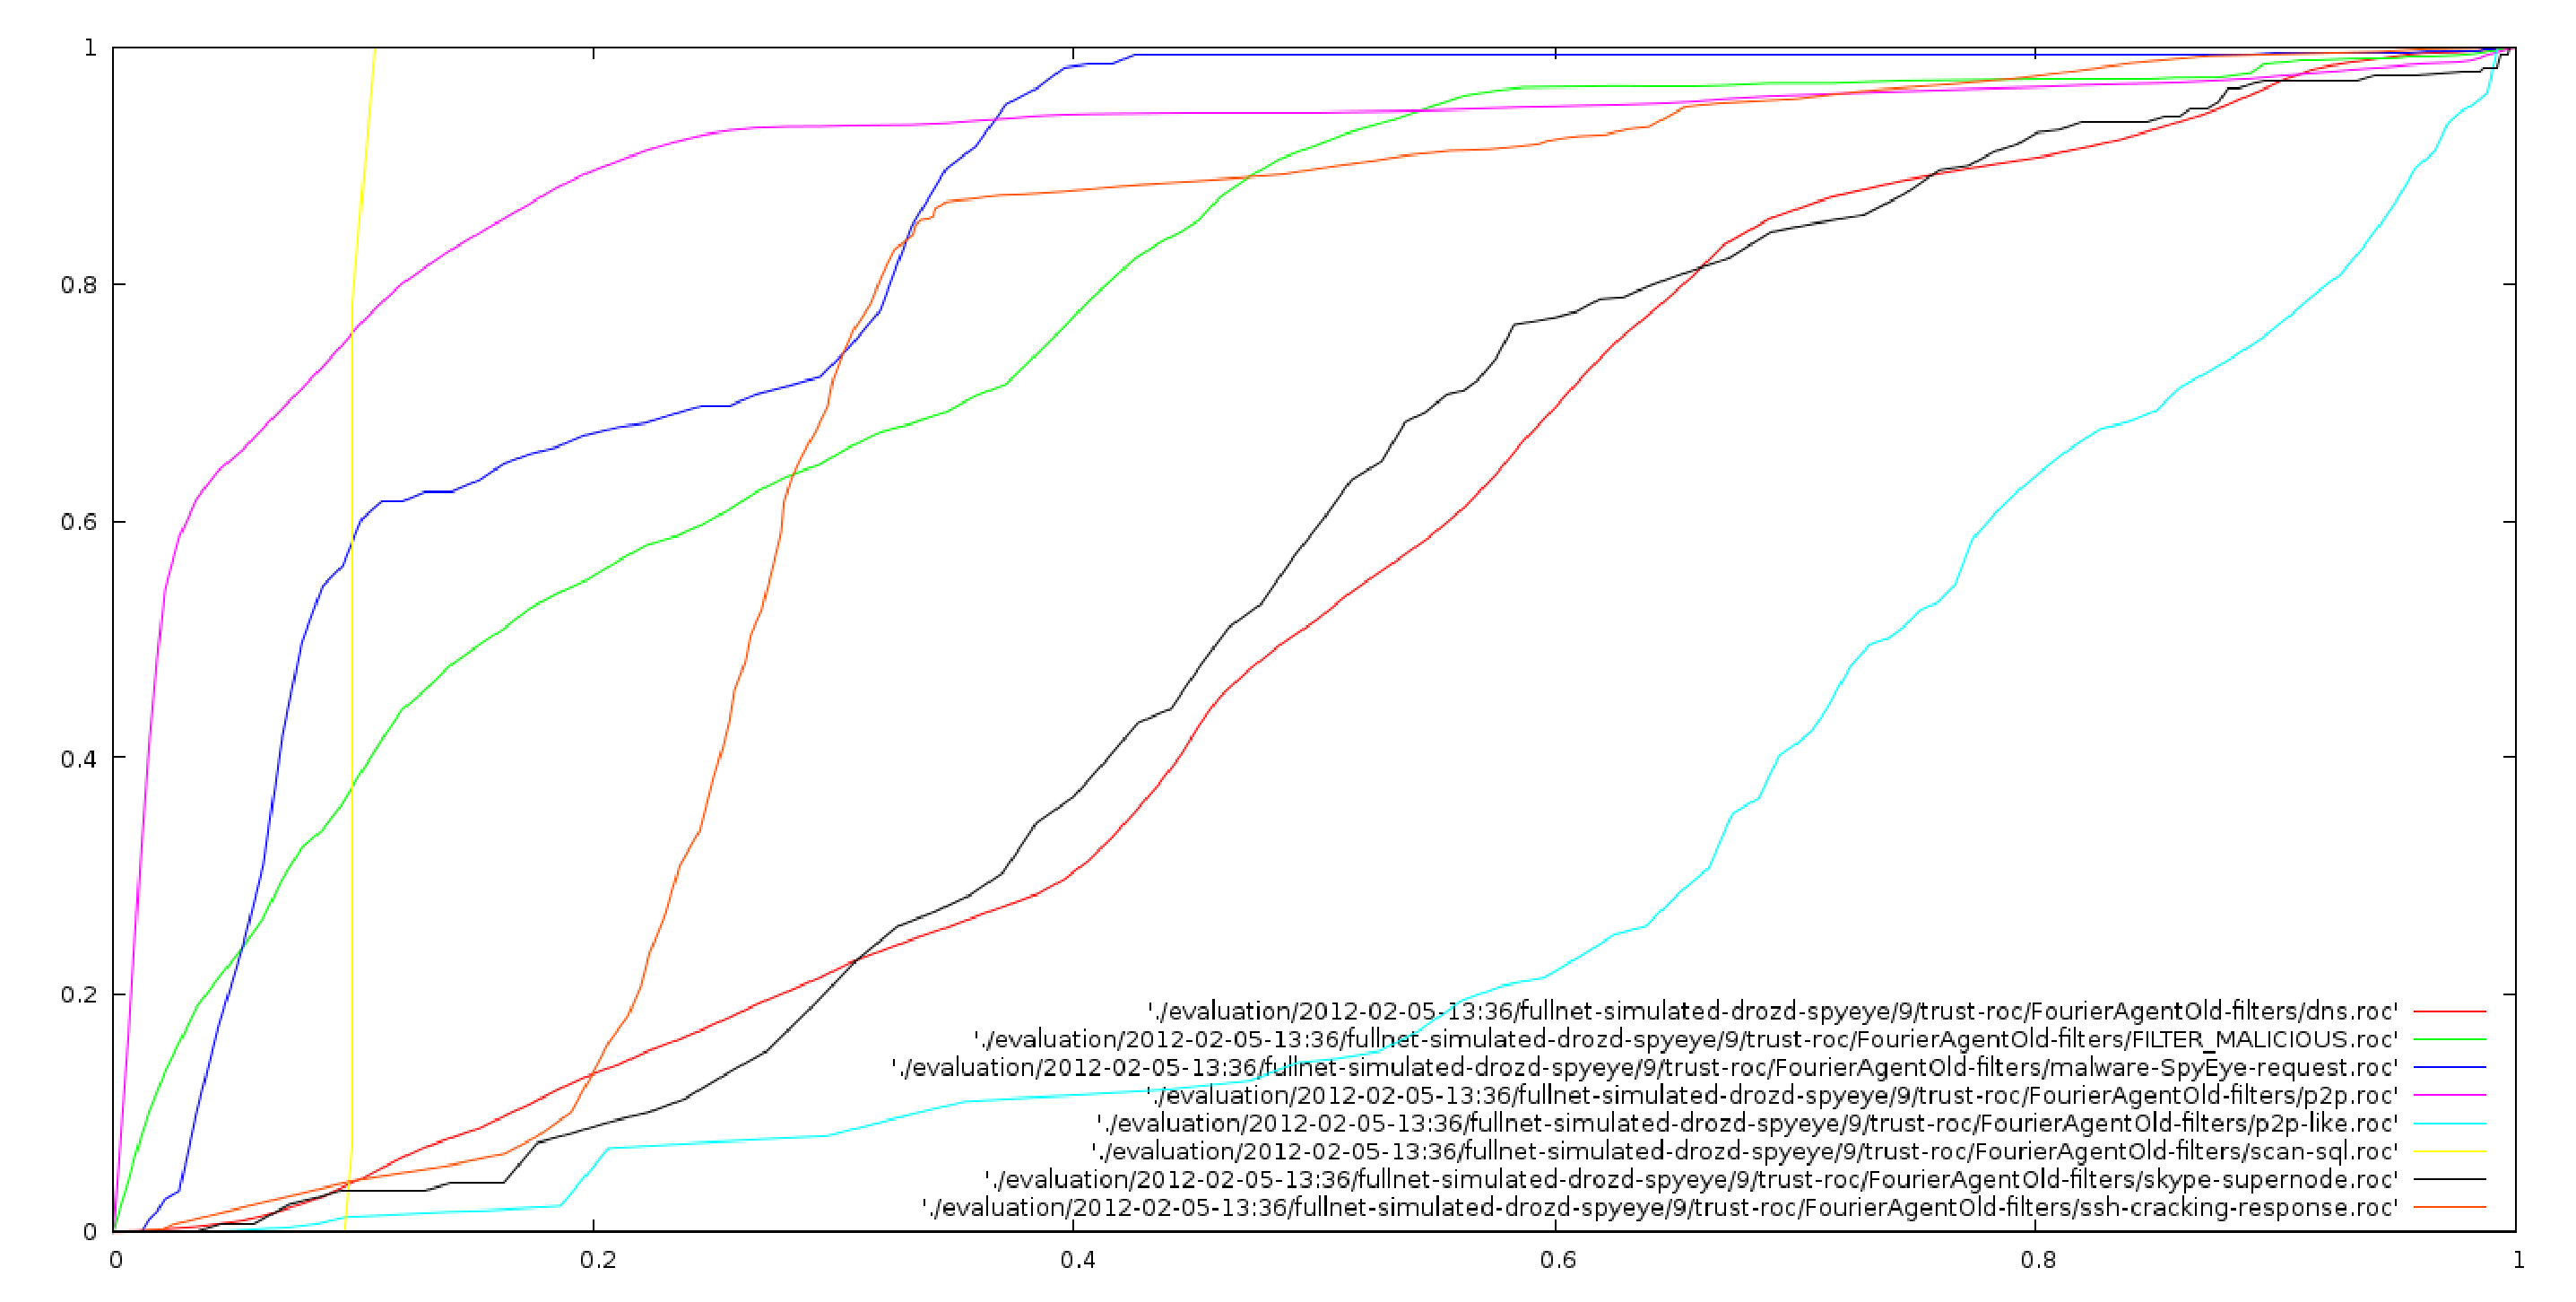
\includegraphics[width=160mm]{old}
%  \caption{NDAFUK}
%  \label{fig:old}
%\end{figure}

% that's all folks
\end{document}
